%orbitas sociologicas, hubs, prediccion global movilidad, forwarding
\subsubsection{SOLAR}
SOLAR \cite{solar} es un protocolo que considera una predicción de la movilidad de los nodos de manera global, dada la dificultad de mantener información detallada de movimientos individuales en DTNs. Considera un patrón de movimiento \emph{orbital} en torno a varios \emph{ejes}, denominado \emph{parcialmente determinista}, a diferencia de movimientos deterministas como satélites o buses considerados en otros protocolos.

El patrón de movimiento orbital considera \emph{hubs} o ejes asociados a un tiempo de estadía, definiendo un conjunto de éstos la Órbita Inter-Ejes (IHO en inglés), considerando así el movimiento dentro de los hubs como entre éstos, los cuales a su vez pueden ser otros patrones de movimiento, como se muestra en la Figura \ref{fig:orbit}

\begin{figure}[h]
\centering
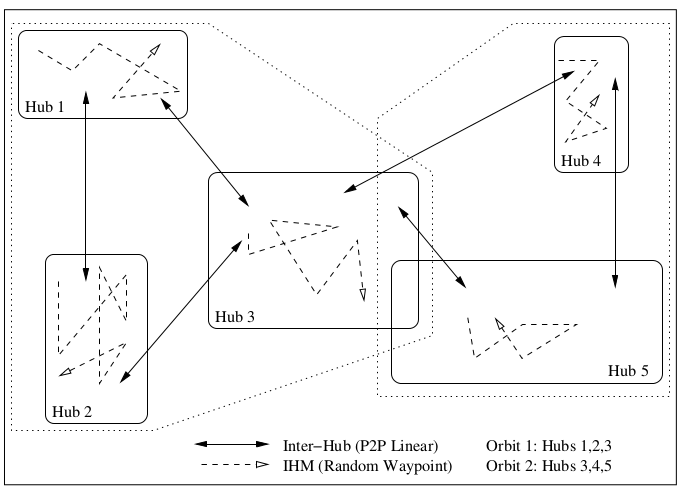
\includegraphics[width=200px]{solar-orbit.png}
\caption{Modelo ORBIT aleatorio \cite{solar}}
\label{fig:orbit}
\end{figure}

Cuando los nodos se encuentran, intercambian sus IHOs en su saludo, volviéndose \emph{conocidos} entre sí. Así, para enrutar, el nodo busca si conoce su IHO. Si lo hace, envía paquetes a sus ejes. Si no, pregunta a sus conocidos si lo conocen, hasta encontrar su IHO. Si además se conoce la posición aproximada de los ejes, se puede utilizar un protocolo geográfico para llegar al destino, que obtiene mejores resultados que otros protocolos.
Decidir el mejor conjunto de nodos \emph{conocidos} es un problema que puede reducirse a \texttt{Set Cover}, que es NP-Hard, volviendo costoso buscar un buen conjunto y debiendo utilizar aproximaciones.
En la implementación simplificada de este protocolo se obtiene desempeño comparable a Epidemic y con menos \emph{overhead}, pero al ser bastante básica deja mucho espacio para mejoras.